\INEchaptercarta{Desigualdad}{}


\cajita{Desigualdad según el índice de Gini}{\textollamada[*]{El índice de gini mide la distancia a la perfecta igualdad. Su valor varía de 0 a 1, entre más cerca de 1, mayor es la desigualdad.} El concepto de desigualdad del ingreso, está relacionado con las diferencias relativas del ingreso entre personas.   

Al observar la participación de los quintiles en el ingreso per cápita familiar, se advierte que entre 2000 y 2014, no ha variado mucho la participación de cada quintil, ya que el quintil más bajo obtiene menos del 3\% de los ingresos y el quintil más alto capta más del 60\% de los ingresos.
}{Índice de Gini }{República de Guatemala, serie histórica por Encovi, adimensional}{\ \\[0mm]\begin{tikzpicture}[x=1pt,y=1pt]  % Created by tikzDevice version 0.7.0 on 2015-11-27 11:21:46
% !TEX encoding = UTF-8 Unicode
\definecolor[named]{fillColor}{rgb}{1.00,1.00,1.00}
\path[use as bounding box,fill=fillColor,fill opacity=0.00] (0,0) rectangle (289.08,198.74);
\begin{scope}
\path[clip] (  0.00,  0.00) rectangle (289.08,198.74);

\path[] (  0.00,  0.00) rectangle (289.08,198.74);
\end{scope}
\begin{scope}
\path[clip] (  0.00,  0.00) rectangle (289.08,198.74);

\path[] ( 12.44, 17.78) rectangle (280.54,191.48);

\path[] ( 12.44, 41.46) --
	(280.54, 41.46);

\path[] ( 12.44, 73.05) --
	(280.54, 73.05);

\path[] ( 12.44,104.63) --
	(280.54,104.63);

\path[] ( 12.44,136.21) --
	(280.54,136.21);

\path[] ( 12.44,167.80) --
	(280.54,167.80);

\path[] ( 12.44, 25.67) --
	(280.54, 25.67);

\path[] ( 12.44, 57.25) --
	(280.54, 57.25);

\path[] ( 12.44, 88.84) --
	(280.54, 88.84);

\path[] ( 12.44,120.42) --
	(280.54,120.42);

\path[] ( 12.44,152.00) --
	(280.54,152.00);

\path[] ( 12.44,183.59) --
	(280.54,183.59);

\path[] ( 50.74, 17.78) --
	( 50.74,191.48);

\path[] (114.57, 17.78) --
	(114.57,191.48);

\path[] (178.41, 17.78) --
	(178.41,191.48);

\path[] (242.24, 17.78) --
	(242.24,191.48);
\definecolor[named]{drawColor}{rgb}{0.00,0.00,1.00}

\path[draw=drawColor,line width= 1.7pt,line join=round] ( 50.74,152.94) --
	(114.57,138.59) --
	(178.41,140.92) --
	(242.24,130.29);
\definecolor[named]{drawColor}{rgb}{0.00,0.00,0.00}

\node[text=drawColor,anchor=base,inner sep=0pt, outer sep=0pt, scale=  1.01] at ( 50.74,156.90) {0.60};

\node[text=drawColor,anchor=base,inner sep=0pt, outer sep=0pt, scale=  1.01] at (114.57,126.72) {0.56};

\node[text=drawColor,anchor=base,inner sep=0pt, outer sep=0pt, scale=  1.01] at (178.41,144.88) {0.56};

\node[text=drawColor,anchor=base,inner sep=0pt, outer sep=0pt, scale=  1.01] at (242.24,118.42) {0.53};
\definecolor[named]{fillColor}{rgb}{0.00,0.00,0.00}

\path[draw=drawColor,line width= 0.1pt,line join=round,fill=fillColor] ( 12.44, 25.67) -- (280.54, 25.67);

\path[] ( 12.44, 17.78) rectangle (280.54,191.48);
\end{scope}
\begin{scope}
\path[clip] (  0.00,  0.00) rectangle (289.08,198.74);

\path[] ( 12.44, 17.78) --
	( 12.44,191.48);
\end{scope}
\begin{scope}
\path[clip] (  0.00,  0.00) rectangle (289.08,198.74);
\definecolor[named]{drawColor}{rgb}{1.00,1.00,1.00}

\node[text=drawColor,text opacity=0.00,anchor=base east,inner sep=0pt, outer sep=0pt, scale=  1.00] at (  5.32, 21.76) {0.2};

\node[text=drawColor,text opacity=0.00,anchor=base east,inner sep=0pt, outer sep=0pt, scale=  1.00] at (  5.32, 53.35) {0.3};

\node[text=drawColor,text opacity=0.00,anchor=base east,inner sep=0pt, outer sep=0pt, scale=  1.00] at (  5.32, 84.93) {0.4};

\node[text=drawColor,text opacity=0.00,anchor=base east,inner sep=0pt, outer sep=0pt, scale=  1.00] at (  5.32,116.51) {0.5};

\node[text=drawColor,text opacity=0.00,anchor=base east,inner sep=0pt, outer sep=0pt, scale=  1.00] at (  5.32,148.10) {0.6};

\node[text=drawColor,text opacity=0.00,anchor=base east,inner sep=0pt, outer sep=0pt, scale=  1.00] at (  5.32,179.68) {0.7};
\end{scope}
\begin{scope}
\path[clip] (  0.00,  0.00) rectangle (289.08,198.74);

\path[] (  8.17, 25.67) --
	( 12.44, 25.67);

\path[] (  8.17, 57.25) --
	( 12.44, 57.25);

\path[] (  8.17, 88.84) --
	( 12.44, 88.84);

\path[] (  8.17,120.42) --
	( 12.44,120.42);

\path[] (  8.17,152.00) --
	( 12.44,152.00);

\path[] (  8.17,183.59) --
	( 12.44,183.59);
\end{scope}
\begin{scope}
\path[clip] (  0.00,  0.00) rectangle (289.08,198.74);

\path[] ( 12.44, 17.78) --
	(280.54, 17.78);
\end{scope}
\begin{scope}
\path[clip] (  0.00,  0.00) rectangle (289.08,198.74);

\path[] ( 50.74, 13.51) --
	( 50.74, 17.78);

\path[] (114.57, 13.51) --
	(114.57, 17.78);

\path[] (178.41, 13.51) --
	(178.41, 17.78);

\path[] (242.24, 13.51) --
	(242.24, 17.78);
\end{scope}
\begin{scope}
\path[clip] (  0.00,  0.00) rectangle (289.08,198.74);
\definecolor[named]{drawColor}{rgb}{0.00,0.00,0.00}

\node[text=drawColor,anchor=base,inner sep=0pt, outer sep=0pt, scale=  1.00] at ( 50.74,  2.85) {2000};

\node[text=drawColor,anchor=base,inner sep=0pt, outer sep=0pt, scale=  1.00] at (114.57,  2.85) {2006};

\node[text=drawColor,anchor=base,inner sep=0pt, outer sep=0pt, scale=  1.00] at (178.41,  2.85) {2011};

\node[text=drawColor,anchor=base,inner sep=0pt, outer sep=0pt, scale=  1.00] at (242.24,  2.85) {2014};
\end{scope}
  \end{tikzpicture}}{}


\cajita{Desigualdad según el índice de Atkinson con $ \varepsilon = 1$}{\textollamada[*]{El índice de Atkinson mide}El concepto de desigualdad del ingreso, está relacionado con las diferencias relativas del ingreso entre personas.   

Al observar la participación de los quintiles en el ingreso per cápita familiar, se advierte que entre 2000 y 2014, no ha variado mucho la participación de cada quintil, ya que el quintil más bajo obtiene menos del 3\% de los ingresos y el quintil más alto capta más del 60\% de los ingresos.
}{Índice de Atkinson, con $ \varepsilon = 1$}{República de Guatemala, serie histórica por Encovi, adimensional}{\ \\[0mm]\begin{tikzpicture}[x=1pt,y=1pt]  % Created by tikzDevice version 0.7.0 on 2015-11-24 06:39:09
% !TEX encoding = UTF-8 Unicode
\definecolor[named]{fillColor}{rgb}{1.00,1.00,1.00}
\path[use as bounding box,fill=fillColor,fill opacity=0.00] (0,0) rectangle (289.08,198.74);
\begin{scope}
\path[clip] (  0.00,  0.00) rectangle (289.08,198.74);

\path[] (  0.00,  0.00) rectangle (289.08,198.74);
\end{scope}
\begin{scope}
\path[clip] (  0.00,  0.00) rectangle (289.08,198.74);

\path[] ( 16.82, 17.78) rectangle (280.54,191.48);

\path[] ( 16.82, 27.01) --
	(280.54, 27.01);

\path[] ( 16.82, 70.85) --
	(280.54, 70.85);

\path[] ( 16.82,114.68) --
	(280.54,114.68);

\path[] ( 16.82,158.52) --
	(280.54,158.52);

\path[] ( 16.82, 48.93) --
	(280.54, 48.93);

\path[] ( 16.82, 92.77) --
	(280.54, 92.77);

\path[] ( 16.82,136.60) --
	(280.54,136.60);

\path[] ( 16.82,180.44) --
	(280.54,180.44);

\path[] ( 54.49, 17.78) --
	( 54.49,191.48);

\path[] (117.28, 17.78) --
	(117.28,191.48);

\path[] (180.08, 17.78) --
	(180.08,191.48);

\path[] (242.87, 17.78) --
	(242.87,191.48);
\definecolor[named]{drawColor}{rgb}{0.00,0.00,1.00}

\path[draw=drawColor,line width= 1.7pt,line join=round] ( 54.49,183.59) --
	(117.28, 99.88) --
	(180.08,103.93) --
	(242.87, 62.11);
\definecolor[named]{drawColor}{rgb}{0.00,0.00,0.00}

\node[text=drawColor,anchor=base,inner sep=0pt, outer sep=0pt, scale=  1.01] at ( 54.49,187.54) {0.52};

\node[text=drawColor,anchor=base,inner sep=0pt, outer sep=0pt, scale=  1.01] at (117.28, 88.01) {0.45};

\node[text=drawColor,anchor=base,inner sep=0pt, outer sep=0pt, scale=  1.01] at (180.08,107.89) {0.45};

\node[text=drawColor,anchor=base,inner sep=0pt, outer sep=0pt, scale=  1.01] at (242.87, 50.24) {0.41};
\definecolor[named]{fillColor}{rgb}{0.00,0.00,0.00}

\path[draw=drawColor,line width= 0.1pt,line join=round,fill=fillColor] ( 16.82, 25.67) -- (280.54, 25.67);

\path[] ( 16.82, 17.78) rectangle (280.54,191.48);
\end{scope}
\begin{scope}
\path[clip] (  0.00,  0.00) rectangle (289.08,198.74);

\path[] ( 16.82, 17.78) --
	( 16.82,191.48);
\end{scope}
\begin{scope}
\path[clip] (  0.00,  0.00) rectangle (289.08,198.74);
\definecolor[named]{drawColor}{rgb}{1.00,1.00,1.00}

\node[text=drawColor,text opacity=0.00,anchor=base east,inner sep=0pt, outer sep=0pt, scale=  1.00] at (  9.70, 45.02) {0.40};

\node[text=drawColor,text opacity=0.00,anchor=base east,inner sep=0pt, outer sep=0pt, scale=  1.00] at (  9.70, 88.86) {0.44};

\node[text=drawColor,text opacity=0.00,anchor=base east,inner sep=0pt, outer sep=0pt, scale=  1.00] at (  9.70,132.69) {0.48};

\node[text=drawColor,text opacity=0.00,anchor=base east,inner sep=0pt, outer sep=0pt, scale=  1.00] at (  9.70,176.53) {0.52};
\end{scope}
\begin{scope}
\path[clip] (  0.00,  0.00) rectangle (289.08,198.74);

\path[] ( 12.55, 48.93) --
	( 16.82, 48.93);

\path[] ( 12.55, 92.77) --
	( 16.82, 92.77);

\path[] ( 12.55,136.60) --
	( 16.82,136.60);

\path[] ( 12.55,180.44) --
	( 16.82,180.44);
\end{scope}
\begin{scope}
\path[clip] (  0.00,  0.00) rectangle (289.08,198.74);

\path[] ( 16.82, 17.78) --
	(280.54, 17.78);
\end{scope}
\begin{scope}
\path[clip] (  0.00,  0.00) rectangle (289.08,198.74);

\path[] ( 54.49, 13.51) --
	( 54.49, 17.78);

\path[] (117.28, 13.51) --
	(117.28, 17.78);

\path[] (180.08, 13.51) --
	(180.08, 17.78);

\path[] (242.87, 13.51) --
	(242.87, 17.78);
\end{scope}
\begin{scope}
\path[clip] (  0.00,  0.00) rectangle (289.08,198.74);
\definecolor[named]{drawColor}{rgb}{0.00,0.00,0.00}

\node[text=drawColor,anchor=base,inner sep=0pt, outer sep=0pt, scale=  1.00] at ( 54.49,  2.85) {2000};

\node[text=drawColor,anchor=base,inner sep=0pt, outer sep=0pt, scale=  1.00] at (117.28,  2.85) {2006};

\node[text=drawColor,anchor=base,inner sep=0pt, outer sep=0pt, scale=  1.00] at (180.08,  2.85) {2011};

\node[text=drawColor,anchor=base,inner sep=0pt, outer sep=0pt, scale=  1.00] at (242.87,  2.85) {2014};
\end{scope}
  \end{tikzpicture}}{ }

\cajita{Desigualdad según el índice de Atkinson con $ \varepsilon = 2$}{\textollamada[*]{El índice de Atkinson mide…. Para e=2…}El concepto de desigualdad del ingreso, está relacionado con las diferencias relativas del ingreso entre personas.   

Al observar la participación de los quintiles en el ingreso per cápita familiar, se advierte que entre 2000 y 2014, no ha variado mucho la participación de cada quintil, ya que el quintil más bajo obtiene menos del 3\% de los ingresos y el quintil más alto capta más del 60\% de los ingresos.
}{Índice de Atkinson, con $ \varepsilon = 2$}{República de Guatemala, serie histórica por Encovi, adimensional}{\ \\[0mm]\begin{tikzpicture}[x=1pt,y=1pt]  % Created by tikzDevice version 0.7.0 on 2015-11-27 11:35:14
% !TEX encoding = UTF-8 Unicode
\definecolor[named]{fillColor}{rgb}{1.00,1.00,1.00}
\path[use as bounding box,fill=fillColor,fill opacity=0.00] (0,0) rectangle (289.08,198.74);
\begin{scope}
\path[clip] (  0.00,  0.00) rectangle (289.08,198.74);

\path[] (  0.00,  0.00) rectangle (289.08,198.74);
\end{scope}
\begin{scope}
\path[clip] (  0.00,  0.00) rectangle (289.08,198.74);

\path[] ( 12.44, 17.78) rectangle (280.54,191.48);

\path[] ( 12.44, 65.15) --
	(280.54, 65.15);

\path[] ( 12.44,117.79) --
	(280.54,117.79);

\path[] ( 12.44,170.43) --
	(280.54,170.43);

\path[] ( 12.44, 38.83) --
	(280.54, 38.83);

\path[] ( 12.44, 91.47) --
	(280.54, 91.47);

\path[] ( 12.44,144.11) --
	(280.54,144.11);

\path[] ( 50.74, 17.78) --
	( 50.74,191.48);

\path[] (114.57, 17.78) --
	(114.57,191.48);

\path[] (178.41, 17.78) --
	(178.41,191.48);

\path[] (242.24, 17.78) --
	(242.24,191.48);
\definecolor[named]{drawColor}{rgb}{0.00,0.00,1.00}

\path[draw=drawColor,line width= 1.7pt,line join=round] ( 50.74,167.92) --
	(114.57,123.44) --
	(178.41,135.13) --
	(242.24,121.56);
\definecolor[named]{drawColor}{rgb}{0.00,0.00,0.00}

\node[text=drawColor,anchor=base,inner sep=0pt, outer sep=0pt, scale=  1.01] at ( 50.74,171.87) {0.89};

\node[text=drawColor,anchor=base,inner sep=0pt, outer sep=0pt, scale=  1.01] at (114.57,111.57) {0.72};

\node[text=drawColor,anchor=base,inner sep=0pt, outer sep=0pt, scale=  1.01] at (178.41,139.09) {0.77};

\node[text=drawColor,anchor=base,inner sep=0pt, outer sep=0pt, scale=  1.01] at (242.24,109.69) {0.71};
\definecolor[named]{fillColor}{rgb}{0.00,0.00,0.00}

\path[draw=drawColor,line width= 0.1pt,line join=round,fill=fillColor] ( 12.44, 25.67) -- (280.54, 25.67);

\path[] ( 12.44, 17.78) rectangle (280.54,191.48);
\end{scope}
\begin{scope}
\path[clip] (  0.00,  0.00) rectangle (289.08,198.74);

\path[] ( 12.44, 17.78) --
	( 12.44,191.48);
\end{scope}
\begin{scope}
\path[clip] (  0.00,  0.00) rectangle (289.08,198.74);
\definecolor[named]{drawColor}{rgb}{1.00,1.00,1.00}

\node[text=drawColor,text opacity=0.00,anchor=base east,inner sep=0pt, outer sep=0pt, scale=  1.00] at (  5.32, 34.92) {0.4};

\node[text=drawColor,text opacity=0.00,anchor=base east,inner sep=0pt, outer sep=0pt, scale=  1.00] at (  5.32, 87.56) {0.6};

\node[text=drawColor,text opacity=0.00,anchor=base east,inner sep=0pt, outer sep=0pt, scale=  1.00] at (  5.32,140.20) {0.8};
\end{scope}
\begin{scope}
\path[clip] (  0.00,  0.00) rectangle (289.08,198.74);

\path[] (  8.17, 38.83) --
	( 12.44, 38.83);

\path[] (  8.17, 91.47) --
	( 12.44, 91.47);

\path[] (  8.17,144.11) --
	( 12.44,144.11);
\end{scope}
\begin{scope}
\path[clip] (  0.00,  0.00) rectangle (289.08,198.74);

\path[] ( 12.44, 17.78) --
	(280.54, 17.78);
\end{scope}
\begin{scope}
\path[clip] (  0.00,  0.00) rectangle (289.08,198.74);

\path[] ( 50.74, 13.51) --
	( 50.74, 17.78);

\path[] (114.57, 13.51) --
	(114.57, 17.78);

\path[] (178.41, 13.51) --
	(178.41, 17.78);

\path[] (242.24, 13.51) --
	(242.24, 17.78);
\end{scope}
\begin{scope}
\path[clip] (  0.00,  0.00) rectangle (289.08,198.74);
\definecolor[named]{drawColor}{rgb}{0.00,0.00,0.00}

\node[text=drawColor,anchor=base,inner sep=0pt, outer sep=0pt, scale=  1.00] at ( 50.74,  2.85) {2000};

\node[text=drawColor,anchor=base,inner sep=0pt, outer sep=0pt, scale=  1.00] at (114.57,  2.85) {2006};

\node[text=drawColor,anchor=base,inner sep=0pt, outer sep=0pt, scale=  1.00] at (178.41,  2.85) {2011};

\node[text=drawColor,anchor=base,inner sep=0pt, outer sep=0pt, scale=  1.00] at (242.24,  2.85) {2014};
\end{scope}
  \end{tikzpicture}}{}

\cajita{Desigualdad según el índice de Theil}{\textollamada[*]{El índice de Theil mide}El concepto de desigualdad del ingreso, está relacionado con las diferencias relativas del ingreso entre personas.   

Al observar la participación de los quintiles en el ingreso per cápita familiar, se advierte que entre 2000 y 2014, no ha variado mucho la participación de cada quintil, ya que el quintil más bajo obtiene menos del 3\% de los ingresos y el quintil más alto capta más del 60\% de los ingresos.
}{Índice de Theil }{República de Guatemala, serie histórica por Encovi, adimensional}{\ \\[0mm]\begin{tikzpicture}[x=1pt,y=1pt]  % Created by tikzDevice version 0.7.0 on 2015-11-27 11:39:26
% !TEX encoding = UTF-8 Unicode
\definecolor[named]{fillColor}{rgb}{1.00,1.00,1.00}
\path[use as bounding box,fill=fillColor,fill opacity=0.00] (0,0) rectangle (289.08,198.74);
\begin{scope}
\path[clip] (  0.00,  0.00) rectangle (289.08,198.74);

\path[] (  0.00,  0.00) rectangle (289.08,198.74);
\end{scope}
\begin{scope}
\path[clip] (  0.00,  0.00) rectangle (289.08,198.74);

\path[] ( 12.44, 17.78) rectangle (280.54,191.48);

\path[] ( 12.44, 41.46) --
	(280.54, 41.46);

\path[] ( 12.44, 73.05) --
	(280.54, 73.05);

\path[] ( 12.44,104.63) --
	(280.54,104.63);

\path[] ( 12.44,136.21) --
	(280.54,136.21);

\path[] ( 12.44,167.80) --
	(280.54,167.80);

\path[] ( 12.44, 25.67) --
	(280.54, 25.67);

\path[] ( 12.44, 57.25) --
	(280.54, 57.25);

\path[] ( 12.44, 88.84) --
	(280.54, 88.84);

\path[] ( 12.44,120.42) --
	(280.54,120.42);

\path[] ( 12.44,152.00) --
	(280.54,152.00);

\path[] ( 12.44,183.59) --
	(280.54,183.59);

\path[] ( 50.74, 17.78) --
	( 50.74,191.48);

\path[] (114.57, 17.78) --
	(114.57,191.48);

\path[] (178.41, 17.78) --
	(178.41,191.48);

\path[] (242.24, 17.78) --
	(242.24,191.48);
\definecolor[named]{drawColor}{rgb}{0.00,0.00,1.00}

\path[draw=drawColor,line width= 1.7pt,line join=round] ( 50.74,172.06) --
	(114.57,127.71) --
	(178.41,161.21) --
	(242.24,118.98);
\definecolor[named]{drawColor}{rgb}{0.00,0.00,0.00}

\node[text=drawColor,anchor=base,inner sep=0pt, outer sep=0pt, scale=  1.01] at ( 50.74,176.01) {0.76};

\node[text=drawColor,anchor=base,inner sep=0pt, outer sep=0pt, scale=  1.01] at (114.57,115.84) {0.62};

\node[text=drawColor,anchor=base,inner sep=0pt, outer sep=0pt, scale=  1.01] at (178.41,165.17) {0.73};

\node[text=drawColor,anchor=base,inner sep=0pt, outer sep=0pt, scale=  1.01] at (242.24,107.11) {0.60};
\definecolor[named]{fillColor}{rgb}{0.00,0.00,0.00}

\path[draw=drawColor,line width= 0.1pt,line join=round,fill=fillColor] ( 12.44, 25.67) -- (280.54, 25.67);

\path[] ( 12.44, 17.78) rectangle (280.54,191.48);
\end{scope}
\begin{scope}
\path[clip] (  0.00,  0.00) rectangle (289.08,198.74);

\path[] ( 12.44, 17.78) --
	( 12.44,191.48);
\end{scope}
\begin{scope}
\path[clip] (  0.00,  0.00) rectangle (289.08,198.74);
\definecolor[named]{drawColor}{rgb}{1.00,1.00,1.00}

\node[text=drawColor,text opacity=0.00,anchor=base east,inner sep=0pt, outer sep=0pt, scale=  1.00] at (  5.32, 21.76) {0.3};

\node[text=drawColor,text opacity=0.00,anchor=base east,inner sep=0pt, outer sep=0pt, scale=  1.00] at (  5.32, 53.35) {0.4};

\node[text=drawColor,text opacity=0.00,anchor=base east,inner sep=0pt, outer sep=0pt, scale=  1.00] at (  5.32, 84.93) {0.5};

\node[text=drawColor,text opacity=0.00,anchor=base east,inner sep=0pt, outer sep=0pt, scale=  1.00] at (  5.32,116.51) {0.6};

\node[text=drawColor,text opacity=0.00,anchor=base east,inner sep=0pt, outer sep=0pt, scale=  1.00] at (  5.32,148.10) {0.7};

\node[text=drawColor,text opacity=0.00,anchor=base east,inner sep=0pt, outer sep=0pt, scale=  1.00] at (  5.32,179.68) {0.8};
\end{scope}
\begin{scope}
\path[clip] (  0.00,  0.00) rectangle (289.08,198.74);

\path[] (  8.17, 25.67) --
	( 12.44, 25.67);

\path[] (  8.17, 57.25) --
	( 12.44, 57.25);

\path[] (  8.17, 88.84) --
	( 12.44, 88.84);

\path[] (  8.17,120.42) --
	( 12.44,120.42);

\path[] (  8.17,152.00) --
	( 12.44,152.00);

\path[] (  8.17,183.59) --
	( 12.44,183.59);
\end{scope}
\begin{scope}
\path[clip] (  0.00,  0.00) rectangle (289.08,198.74);

\path[] ( 12.44, 17.78) --
	(280.54, 17.78);
\end{scope}
\begin{scope}
\path[clip] (  0.00,  0.00) rectangle (289.08,198.74);

\path[] ( 50.74, 13.51) --
	( 50.74, 17.78);

\path[] (114.57, 13.51) --
	(114.57, 17.78);

\path[] (178.41, 13.51) --
	(178.41, 17.78);

\path[] (242.24, 13.51) --
	(242.24, 17.78);
\end{scope}
\begin{scope}
\path[clip] (  0.00,  0.00) rectangle (289.08,198.74);
\definecolor[named]{drawColor}{rgb}{0.00,0.00,0.00}

\node[text=drawColor,anchor=base,inner sep=0pt, outer sep=0pt, scale=  1.00] at ( 50.74,  2.85) {2000};

\node[text=drawColor,anchor=base,inner sep=0pt, outer sep=0pt, scale=  1.00] at (114.57,  2.85) {2006};

\node[text=drawColor,anchor=base,inner sep=0pt, outer sep=0pt, scale=  1.00] at (178.41,  2.85) {2011};

\node[text=drawColor,anchor=base,inner sep=0pt, outer sep=0pt, scale=  1.00] at (242.24,  2.85) {2014};
\end{scope}
  \end{tikzpicture}}{}

\cajita{Participación del quintil más bajo}{\textollamada[*]{Los quintiles se calculan…}El concepto de desigualdad del ingreso, está relacionado con las diferencias relativas del ingreso entre personas.   

Al observar la participación de los quintiles en el ingreso per cápita familiar, se advierte que entre 2000 y 2014, no ha variado mucho la participación de cada quintil, ya que el quintil más bajo obtiene menos del 3\% de los ingresos y el quintil más alto capta más del 60\% de los ingresos.
}{Proporción del primer quintil de ingresos respecto del ingreso total}{República de Guatemala, serie histórica por Encovi, en porcentaje}{\ \\[0mm]\begin{tikzpicture}[x=1pt,y=1pt]  % Created by tikzDevice version 0.9 on 2015-11-26 22:30:54
% !TEX encoding = UTF-8 Unicode
\definecolor{fillColor}{RGB}{255,255,255}
\path[use as bounding box,fill=fillColor,fill opacity=0.00] (0,0) rectangle (289.08,198.74);
\begin{scope}
\path[clip] (  0.00,  0.00) rectangle (289.08,198.74);

\path[] (  0.00,  0.00) rectangle (289.08,198.74);
\end{scope}
\begin{scope}
\path[clip] (  0.00,  0.00) rectangle (289.08,198.74);

\path[] ( 12.44, 17.78) rectangle (280.54,191.48);

\path[] ( 12.44, 41.38) --
	(280.54, 41.38);

\path[] ( 12.44, 88.16) --
	(280.54, 88.16);

\path[] ( 12.44,134.93) --
	(280.54,134.93);

\path[] ( 12.44,181.71) --
	(280.54,181.71);

\path[] ( 12.44, 18.00) --
	(280.54, 18.00);

\path[] ( 12.44, 64.77) --
	(280.54, 64.77);

\path[] ( 12.44,111.55) --
	(280.54,111.55);

\path[] ( 12.44,158.32) --
	(280.54,158.32);

\path[] ( 50.74, 17.78) --
	( 50.74,191.48);

\path[] (114.57, 17.78) --
	(114.57,191.48);

\path[] (178.41, 17.78) --
	(178.41,191.48);

\path[] (242.24, 17.78) --
	(242.24,191.48);
\definecolor{drawColor}{RGB}{0,0,255}

\path[draw=drawColor,line width= 1.7pt,line join=round] ( 50.74, 62.11) --
	(114.57,129.49) --
	(178.41,153.19) --
	(242.24,183.59);
\definecolor{drawColor}{RGB}{0,0,0}

\node[text=drawColor,anchor=base,inner sep=0pt, outer sep=0pt, scale=  1.01] at ( 50.74, 50.24) {2.0};

\node[text=drawColor,anchor=base east,inner sep=0pt, outer sep=0pt, scale=  1.01] at (112.34,129.49) {2.7};

\node[text=drawColor,anchor=base east,inner sep=0pt, outer sep=0pt, scale=  1.01] at (176.18,153.19) {2.9};

\node[text=drawColor,anchor=base,inner sep=0pt, outer sep=0pt, scale=  1.01] at (242.24,187.54) {3.3};

\path[draw=drawColor,line width= 0.1pt,line join=round] ( 12.44, 25.67) -- (280.54, 25.67);

\path[] ( 12.44, 17.78) rectangle (280.54,191.48);
\end{scope}
\begin{scope}
\path[clip] (  0.00,  0.00) rectangle (289.08,198.74);

\path[] ( 12.44, 17.78) --
	( 12.44,191.48);
\end{scope}
\begin{scope}
\path[clip] (  0.00,  0.00) rectangle (289.08,198.74);
\definecolor{drawColor}{RGB}{255,255,255}

\node[text=drawColor,text opacity=0.00,anchor=base east,inner sep=0pt, outer sep=0pt, scale=  1.00] at (  5.32, 14.09) {1.5};

\node[text=drawColor,text opacity=0.00,anchor=base east,inner sep=0pt, outer sep=0pt, scale=  1.00] at (  5.32, 60.86) {2.0};

\node[text=drawColor,text opacity=0.00,anchor=base east,inner sep=0pt, outer sep=0pt, scale=  1.00] at (  5.32,107.64) {2.5};

\node[text=drawColor,text opacity=0.00,anchor=base east,inner sep=0pt, outer sep=0pt, scale=  1.00] at (  5.32,154.41) {3.0};
\end{scope}
\begin{scope}
\path[clip] (  0.00,  0.00) rectangle (289.08,198.74);

\path[] (  8.17, 18.00) --
	( 12.44, 18.00);

\path[] (  8.17, 64.77) --
	( 12.44, 64.77);

\path[] (  8.17,111.55) --
	( 12.44,111.55);

\path[] (  8.17,158.32) --
	( 12.44,158.32);
\end{scope}
\begin{scope}
\path[clip] (  0.00,  0.00) rectangle (289.08,198.74);

\path[] ( 12.44, 17.78) --
	(280.54, 17.78);
\end{scope}
\begin{scope}
\path[clip] (  0.00,  0.00) rectangle (289.08,198.74);

\path[] ( 50.74, 13.51) --
	( 50.74, 17.78);

\path[] (114.57, 13.51) --
	(114.57, 17.78);

\path[] (178.41, 13.51) --
	(178.41, 17.78);

\path[] (242.24, 13.51) --
	(242.24, 17.78);
\end{scope}
\begin{scope}
\path[clip] (  0.00,  0.00) rectangle (289.08,198.74);
\definecolor{drawColor}{RGB}{0,0,0}

\node[text=drawColor,anchor=base,inner sep=0pt, outer sep=0pt, scale=  1.00] at ( 50.74,  2.85) {2000};

\node[text=drawColor,anchor=base,inner sep=0pt, outer sep=0pt, scale=  1.00] at (114.57,  2.85) {2006};

\node[text=drawColor,anchor=base,inner sep=0pt, outer sep=0pt, scale=  1.00] at (178.41,  2.85) {2011};

\node[text=drawColor,anchor=base,inner sep=0pt, outer sep=0pt, scale=  1.00] at (242.24,  2.85) {2014};
\end{scope}
  \end{tikzpicture}}{}

\cajita{Participación del quintil más alto}{\textollamada[*]{Los quintiles se calculan…}El concepto de desigualdad del ingreso, está relacionado con las diferencias relativas del ingreso entre personas.   

Al observar la participación de los quintiles en el ingreso per cápita familiar, se advierte que entre 2000 y 2014, no ha variado mucho la participación de cada quintil, ya que el quintil más bajo obtiene menos del 3\% de los ingresos y el quintil más alto capta más del 60\% de los ingresos.
}{Proporción del quinto quintil de ingresos respecto del ingreso total}{República de Guatemala, serie histórica por Encovi, en porcentaje}{\ \\[0mm]\begin{tikzpicture}[x=1pt,y=1pt]  % Created by tikzDevice version 0.7.0 on 2015-11-24 06:39:17
% !TEX encoding = UTF-8 Unicode
\definecolor[named]{fillColor}{rgb}{1.00,1.00,1.00}
\path[use as bounding box,fill=fillColor,fill opacity=0.00] (0,0) rectangle (289.08,198.74);
\begin{scope}
\path[clip] (  0.00,  0.00) rectangle (289.08,198.74);

\path[] (  0.00,  0.00) rectangle (289.08,198.74);
\end{scope}
\begin{scope}
\path[clip] (  0.00,  0.00) rectangle (289.08,198.74);

\path[] (  8.28, 17.78) rectangle (280.54,191.48);

\path[] (  8.28, 42.22) --
	(280.54, 42.22);

\path[] (  8.28, 88.73) --
	(280.54, 88.73);

\path[] (  8.28,135.23) --
	(280.54,135.23);

\path[] (  8.28,181.74) --
	(280.54,181.74);

\path[] (  8.28, 18.97) --
	(280.54, 18.97);

\path[] (  8.28, 65.48) --
	(280.54, 65.48);

\path[] (  8.28,111.98) --
	(280.54,111.98);

\path[] (  8.28,158.49) --
	(280.54,158.49);

\path[] ( 47.17, 17.78) --
	( 47.17,191.48);

\path[] (112.00, 17.78) --
	(112.00,191.48);

\path[] (176.82, 17.78) --
	(176.82,191.48);

\path[] (241.65, 17.78) --
	(241.65,191.48);
\definecolor[named]{drawColor}{rgb}{0.00,0.00,1.00}

\path[draw=drawColor,line width= 1.7pt,line join=round] ( 47.17,183.59) --
	(112.00,102.34) --
	(176.82,121.31) --
	(241.65, 62.11);
\definecolor[named]{drawColor}{rgb}{0.00,0.00,0.00}

\node[text=drawColor,anchor=base,inner sep=0pt, outer sep=0pt, scale=  1.01] at ( 47.17,187.54) {63.8};

\node[text=drawColor,anchor=base,inner sep=0pt, outer sep=0pt, scale=  1.01] at (112.00, 90.47) {59.5};

\node[text=drawColor,anchor=base,inner sep=0pt, outer sep=0pt, scale=  1.01] at (176.82,125.27) {60.5};

\node[text=drawColor,anchor=base,inner sep=0pt, outer sep=0pt, scale=  1.01] at (241.65, 50.24) {57.3};
\definecolor[named]{fillColor}{rgb}{0.00,0.00,0.00}

\path[draw=drawColor,line width= 0.1pt,line join=round,fill=fillColor] (  8.28, 25.67) -- (280.54, 25.67);

\path[] (  8.28, 17.78) rectangle (280.54,191.48);
\end{scope}
\begin{scope}
\path[clip] (  0.00,  0.00) rectangle (289.08,198.74);

\path[] (  8.28, 17.78) --
	(  8.28,191.48);
\end{scope}
\begin{scope}
\path[clip] (  0.00,  0.00) rectangle (289.08,198.74);
\definecolor[named]{drawColor}{rgb}{1.00,1.00,1.00}

\node[text=drawColor,text opacity=0.00,anchor=base east,inner sep=0pt, outer sep=0pt, scale=  1.00] at (  1.17, 15.06) {55.0};

\node[text=drawColor,text opacity=0.00,anchor=base east,inner sep=0pt, outer sep=0pt, scale=  1.00] at (  1.17, 61.57) {57.5};

\node[text=drawColor,text opacity=0.00,anchor=base east,inner sep=0pt, outer sep=0pt, scale=  1.00] at (  1.17,108.07) {60.0};

\node[text=drawColor,text opacity=0.00,anchor=base east,inner sep=0pt, outer sep=0pt, scale=  1.00] at (  1.17,154.58) {62.5};
\end{scope}
\begin{scope}
\path[clip] (  0.00,  0.00) rectangle (289.08,198.74);

\path[] (  4.01, 18.97) --
	(  8.28, 18.97);

\path[] (  4.01, 65.48) --
	(  8.28, 65.48);

\path[] (  4.01,111.98) --
	(  8.28,111.98);

\path[] (  4.01,158.49) --
	(  8.28,158.49);
\end{scope}
\begin{scope}
\path[clip] (  0.00,  0.00) rectangle (289.08,198.74);

\path[] (  8.28, 17.78) --
	(280.54, 17.78);
\end{scope}
\begin{scope}
\path[clip] (  0.00,  0.00) rectangle (289.08,198.74);

\path[] ( 47.17, 13.51) --
	( 47.17, 17.78);

\path[] (112.00, 13.51) --
	(112.00, 17.78);

\path[] (176.82, 13.51) --
	(176.82, 17.78);

\path[] (241.65, 13.51) --
	(241.65, 17.78);
\end{scope}
\begin{scope}
\path[clip] (  0.00,  0.00) rectangle (289.08,198.74);
\definecolor[named]{drawColor}{rgb}{0.00,0.00,0.00}

\node[text=drawColor,anchor=base,inner sep=0pt, outer sep=0pt, scale=  1.00] at ( 47.17,  2.85) {2000};

\node[text=drawColor,anchor=base,inner sep=0pt, outer sep=0pt, scale=  1.00] at (112.00,  2.85) {2006};

\node[text=drawColor,anchor=base,inner sep=0pt, outer sep=0pt, scale=  1.00] at (176.82,  2.85) {2011};

\node[text=drawColor,anchor=base,inner sep=0pt, outer sep=0pt, scale=  1.00] at (241.65,  2.85) {2014};
\end{scope}
  \end{tikzpicture}}{}

\cajita{Relación de ingresos del quintil más alto y más bajo}{\textollamada[*]{Los quintiles se calculan…} El concepto de desigualdad del ingreso, está relacionado con las diferencias relativas del ingreso entre personas.   

Al observar la participación de los quintiles en el ingreso per cápita familiar, se advierte que entre 2000 y 2014, no ha variado mucho la participación de cada quintil, ya que el quintil más bajo obtiene menos del 3\% de los ingresos y el quintil más alto capta más del 60\% de los ingresos.}{Razón del quinto y primer quintil de ingresos}{República de Guatemala, serie histórica por Encovi, en porcentaje}{\ \\[0mm]\begin{tikzpicture}[x=1pt,y=1pt]  % Created by tikzDevice version 0.7.0 on 2015-11-27 11:45:03
% !TEX encoding = UTF-8 Unicode
\definecolor[named]{fillColor}{rgb}{1.00,1.00,1.00}
\path[use as bounding box,fill=fillColor,fill opacity=0.00] (0,0) rectangle (289.08,198.74);
\begin{scope}
\path[clip] (  0.00,  0.00) rectangle (289.08,198.74);

\path[] (  0.00,  0.00) rectangle (289.08,198.74);
\end{scope}
\begin{scope}
\path[clip] (  0.00,  0.00) rectangle (289.08,198.74);

\path[] (  1.64, 17.78) rectangle (280.54,191.48);

\path[] (  1.64, 41.46) --
	(280.54, 41.46);

\path[] (  1.64, 73.05) --
	(280.54, 73.05);

\path[] (  1.64,104.63) --
	(280.54,104.63);

\path[] (  1.64,136.21) --
	(280.54,136.21);

\path[] (  1.64,167.80) --
	(280.54,167.80);

\path[] (  1.64, 25.67) --
	(280.54, 25.67);

\path[] (  1.64, 57.25) --
	(280.54, 57.25);

\path[] (  1.64, 88.84) --
	(280.54, 88.84);

\path[] (  1.64,120.42) --
	(280.54,120.42);

\path[] (  1.64,152.00) --
	(280.54,152.00);

\path[] (  1.64,183.59) --
	(280.54,183.59);

\path[] ( 41.49, 17.78) --
	( 41.49,191.48);

\path[] (107.89, 17.78) --
	(107.89,191.48);

\path[] (174.30, 17.78) --
	(174.30,191.48);

\path[] (240.70, 17.78) --
	(240.70,191.48);
\definecolor[named]{drawColor}{rgb}{0.00,0.00,1.00}

\path[draw=drawColor,line width= 1.7pt,line join=round] ( 41.49,167.07) --
	(107.89,102.08) --
	(174.30, 92.27) --
	(240.70, 73.23);
\definecolor[named]{drawColor}{rgb}{0.00,0.00,0.00}

\node[text=drawColor,anchor=base,inner sep=0pt, outer sep=0pt, scale=  1.01] at ( 41.49,171.02) {32.4};

\node[text=drawColor,anchor=base west,inner sep=0pt, outer sep=0pt, scale=  1.01] at (107.89,106.04) {22.1};

\node[text=drawColor,anchor=base west,inner sep=0pt, outer sep=0pt, scale=  1.01] at (174.30, 96.22) {20.5};

\node[text=drawColor,anchor=base,inner sep=0pt, outer sep=0pt, scale=  1.01] at (240.70, 61.36) {17.5};
\definecolor[named]{fillColor}{rgb}{0.00,0.00,0.00}

\path[draw=drawColor,line width= 0.1pt,line join=round,fill=fillColor] (  1.64, 25.67) -- (280.54, 25.67);

\path[] (  1.64, 17.78) rectangle (280.54,191.48);
\end{scope}
\begin{scope}
\path[clip] (  0.00,  0.00) rectangle (289.08,198.74);

\path[] (  1.64, 17.78) --
	(  1.64,191.48);
\end{scope}
\begin{scope}
\path[clip] (  0.00,  0.00) rectangle (289.08,198.74);

\path[] (  0.00, 25.67) --
	(  1.64, 25.67);

\path[] (  0.00, 57.25) --
	(  1.64, 57.25);

\path[] (  0.00, 88.84) --
	(  1.64, 88.84);

\path[] (  0.00,120.42) --
	(  1.64,120.42);

\path[] (  0.00,152.00) --
	(  1.64,152.00);

\path[] (  0.00,183.59) --
	(  1.64,183.59);
\end{scope}
\begin{scope}
\path[clip] (  0.00,  0.00) rectangle (289.08,198.74);

\path[] (  1.64, 17.78) --
	(280.54, 17.78);
\end{scope}
\begin{scope}
\path[clip] (  0.00,  0.00) rectangle (289.08,198.74);

\path[] ( 41.49, 13.51) --
	( 41.49, 17.78);

\path[] (107.89, 13.51) --
	(107.89, 17.78);

\path[] (174.30, 13.51) --
	(174.30, 17.78);

\path[] (240.70, 13.51) --
	(240.70, 17.78);
\end{scope}
\begin{scope}
\path[clip] (  0.00,  0.00) rectangle (289.08,198.74);
\definecolor[named]{drawColor}{rgb}{0.00,0.00,0.00}

\node[text=drawColor,anchor=base,inner sep=0pt, outer sep=0pt, scale=  1.00] at ( 41.49,  2.85) {2000};

\node[text=drawColor,anchor=base,inner sep=0pt, outer sep=0pt, scale=  1.00] at (107.89,  2.85) {2006};

\node[text=drawColor,anchor=base,inner sep=0pt, outer sep=0pt, scale=  1.00] at (174.30,  2.85) {2011};

\node[text=drawColor,anchor=base,inner sep=0pt, outer sep=0pt, scale=  1.00] at (240.70,  2.85) {2014};
\end{scope}
  \end{tikzpicture}}{}


\cajota{Desigualdad según el índice Gini en los departamentos}{La desigualdad es mayor en los departamentos }{Índice de Gini }{Por departamento, año 2014, adimensional}{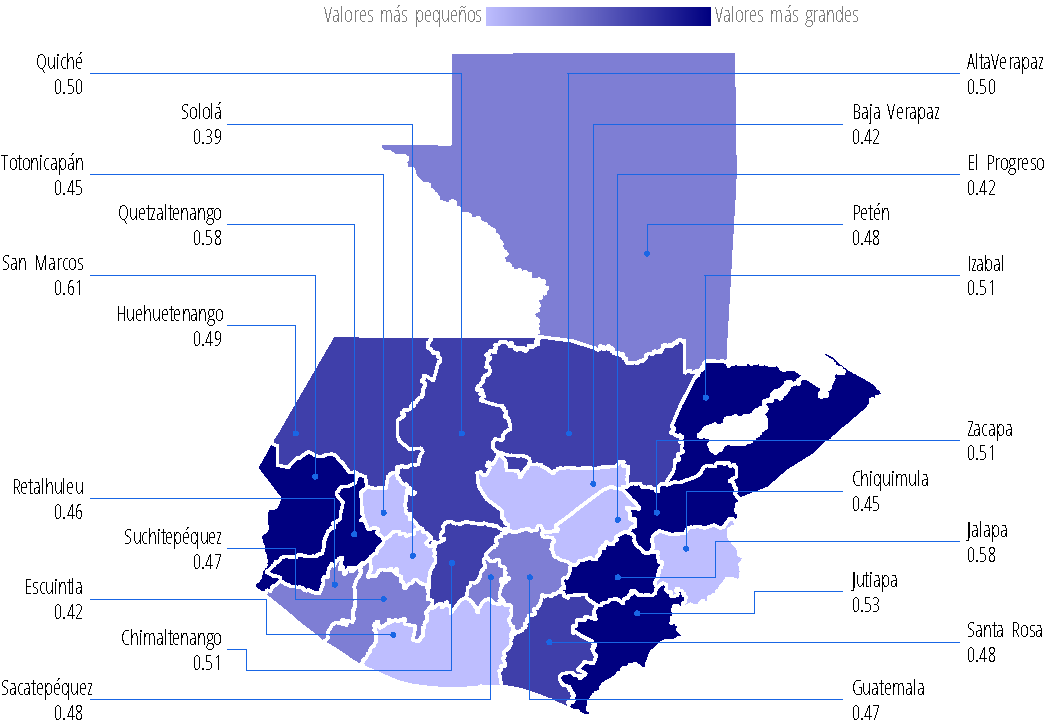
\includegraphics[width=52\cuadri]{graficas/2_08.pdf}}{}

\cajota{Desigualdad en los departamentos según el índice de Atkinson, $ \varepsilon = 1$}{Al desagregar, se observa que los departamentos con mayores niveles de desigualdad son}{Índice de Atkinson con $ \varepsilon = 1$}{Por departamento, año 2014, adimensional}{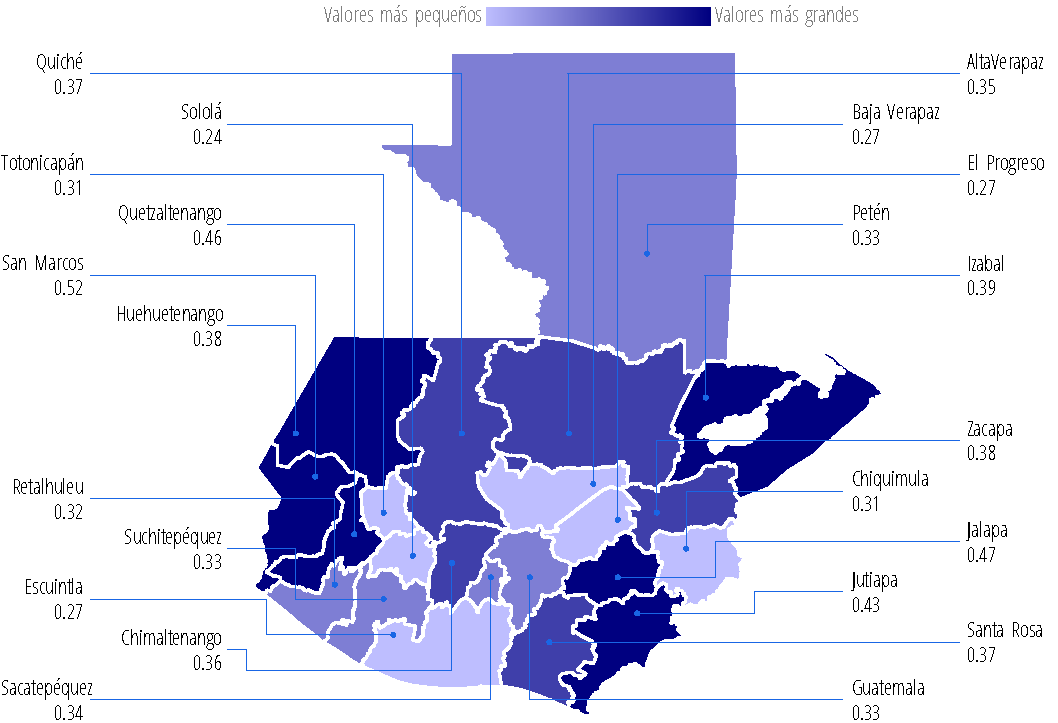
\includegraphics[width=52\cuadri]{graficas/2_09.pdf}  }{}

\cajota{Desigualdad en los departamentos según el índice de Atkinson, $ \varepsilon = 2$}{Al desagregar, se observa que los departamentos con mayores niveles de desigualdad son}{Índice de Atkinson con $ \varepsilon = 2$}{Por departamento, año 2014, adimensional}{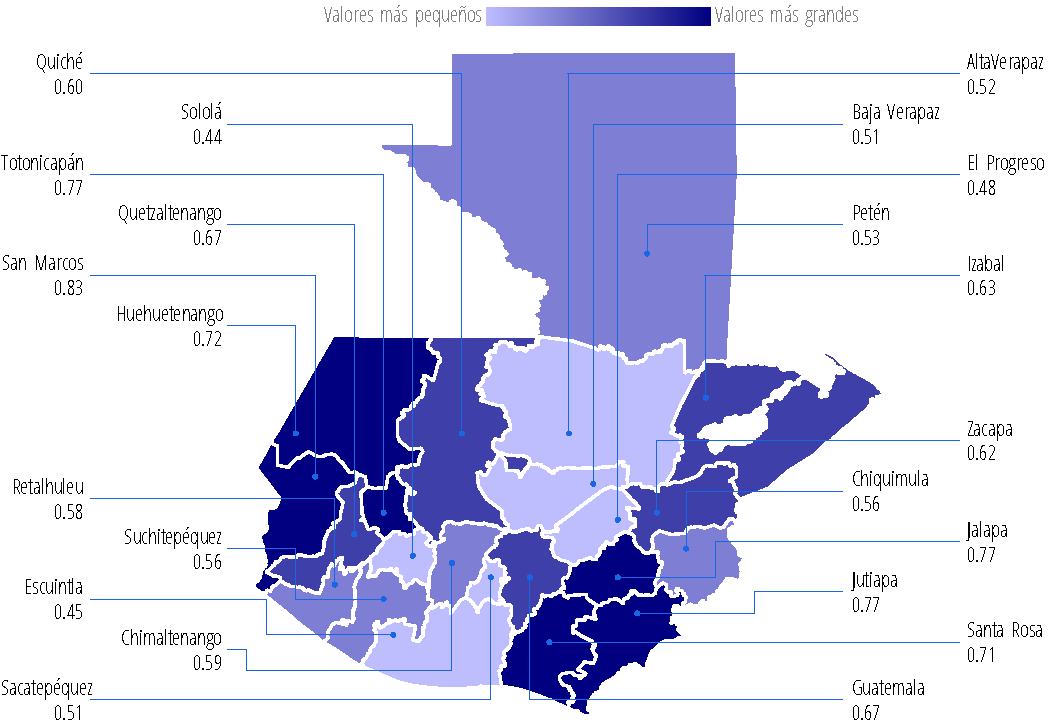
\includegraphics[width=52\cuadri]{graficas/2_10.pdf}  }{}

\cajota{Desigualdad en los departamentos según el índice de Theil}{Al desagregar, se observa que los departamentos con mayores niveles de desigualdad son}{Índice de Theil }{Por departamento, año 2014, adimensional}{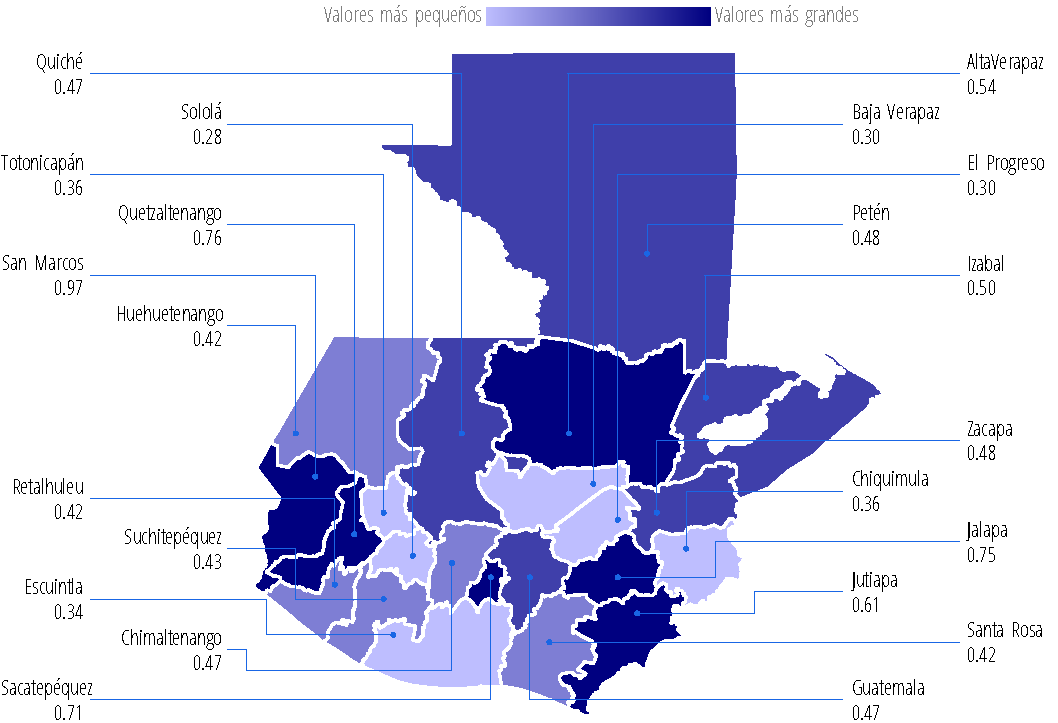
\includegraphics[width=52\cuadri]{graficas/2_11.pdf}  }{}

\cajota{Participación del quintil más bajo en los departamentos}{Al desagregar, se observa que los departamentos con mayores niveles de desigualdad son}{Proporción del primer quintil de ingresos respecto del ingreso total}{Por departamento, año 2014,  en porcentaje}{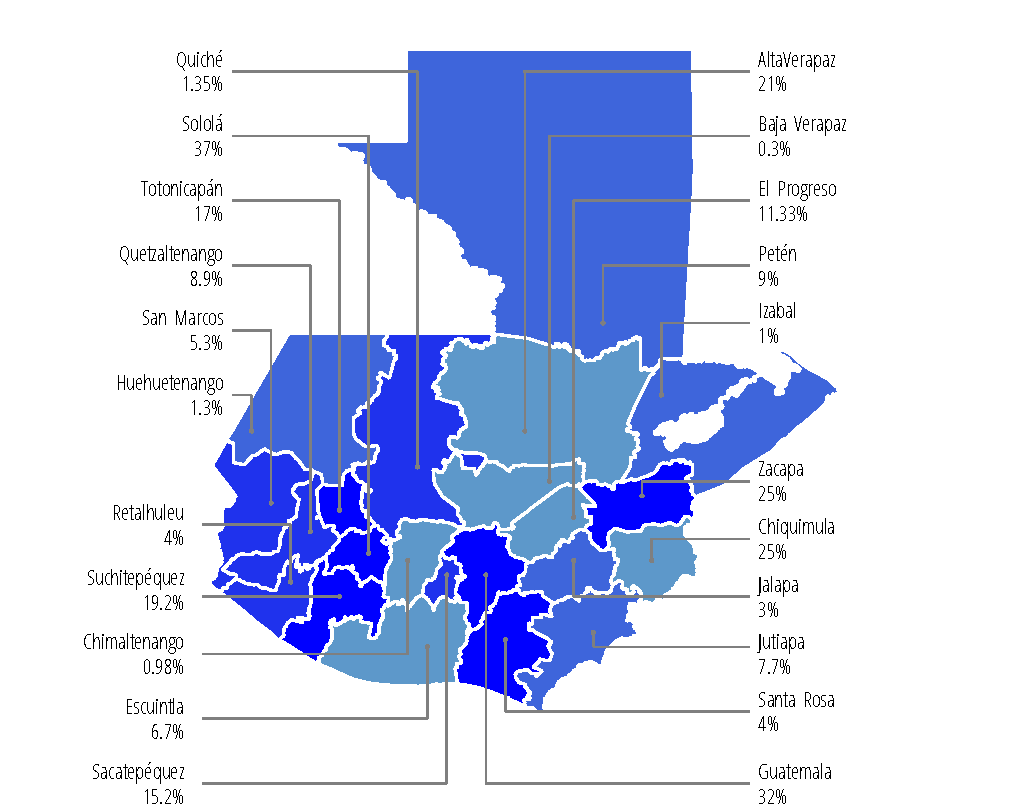
\includegraphics[width=52\cuadri]{graficas/2_12.pdf}  }{}

\cajota{Participación del quintil más alto en los departamentos}{Al desagregar, se observa que los departamentos con mayores niveles de desigualdad son}{Proporción del quinto quintil de ingresos respecto del ingreso total}{Por departamento, año 2014, en porcentaje}{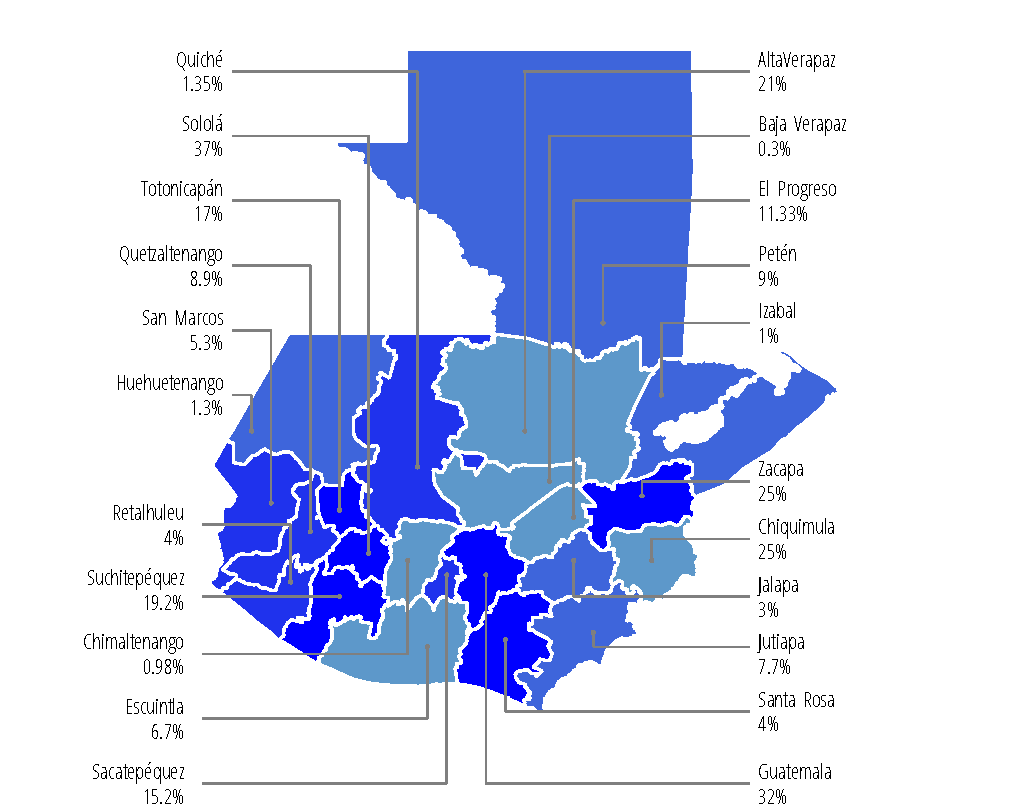
\includegraphics[width=52\cuadri]{graficas/2_13.pdf}  }{}

\cajota{Relación de ingresos del quintil más alto y más bajo en los departamentos}{Al desagregar, se observa que los departamentos con mayores niveles de desigualdad son}{Razón del quinto y primer quintil de ingresos}{Por departamento, año 2014, en porcentaje}{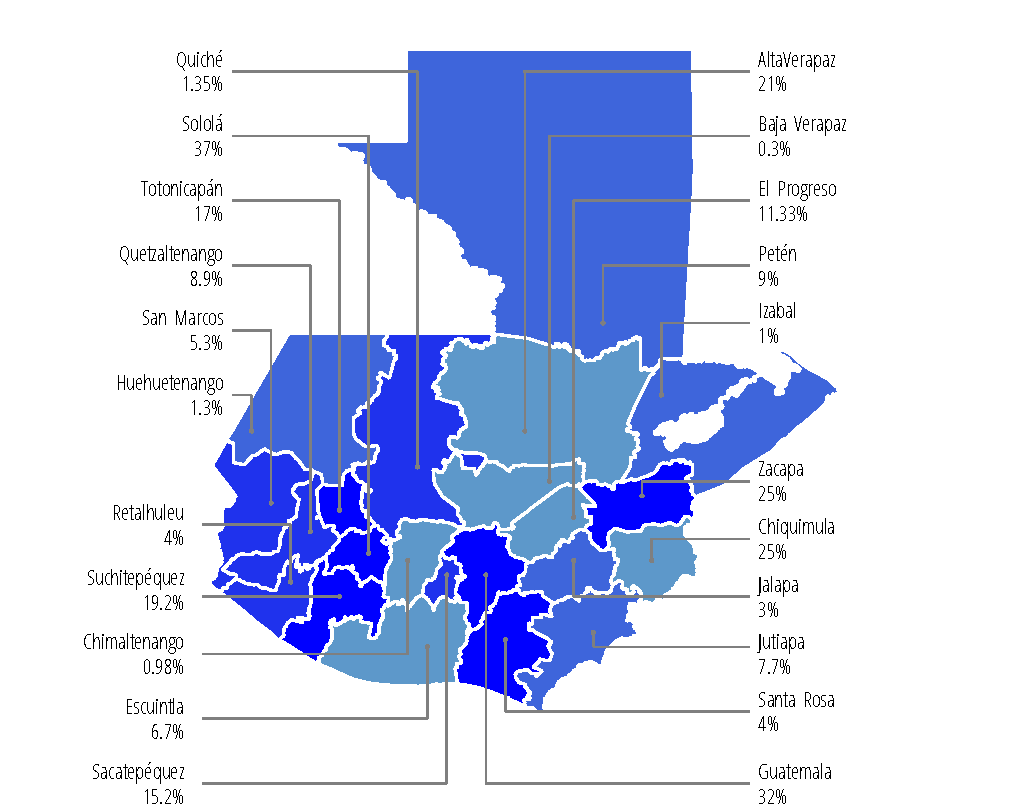
\includegraphics[width=52\cuadri]{graficas/2_14.pdf}  }{}